\documentclass[a4paper,12pt]{article}
%--------------Paquetes---------------------------------------------------------
\usepackage[spanish]{babel}
\usepackage{tikz}
\usepackage{setspace}
\usepackage{eso-pic}
\usepackage{lipsum}
\usepackage{lmodern}
\usepackage{graphicx}
\usepackage[left=25mm, right=25mm, top=35mm, bottom=20mm,headheight=35mm] {geometry}
\usepackage{lastpage}
\usepackage{xcolor}
\usepackage{fancyhdr}
\usepackage{amssymb, amsmath}
\usepackage{float}

\renewcommand*{\familydefault}{\sfdefault}
\graphicspath{./figuras/}
\definecolor{verde}{RGB}{47,97,101}
\pagestyle{fancy}
\renewcommand{\headrulewidth}{2pt}
\let\oldheadrule\headrule
\renewcommand{\headrule}{\color{verde}\oldheadrule}
\lhead{
\includegraphics[width=0.45\textwidth]{figuras/color_UNC-FCEFyN}}
\chead{}
\rfoot{\proyecto}
\rhead{}
%\cfoot{}
%---------------------------------------------------------------------------
%declaro "variables"--------------------------------------------------------
\newcommand{\autor}{Valdez Benavidez, Mauricio L.}
\newcommand{\proyecto}{Trabajo Práctico de Laboratorio N°1}
%\newcommand{\fecha}{\today}

%comienzo del documento----------------------------------------------------
\begin{document}
		\begin{titlepage}
	\newgeometry{left=2.5cm,top=1cm,bottom=2.5cm, right=2.5cm}
	\AddToShipoutPicture*{\put(0,0){
\includegraphics[scale=1]{figuras/background}}} % Image background
	\noindent
	\vspace{1mm}
	{
\includegraphics[width=1\textwidth]{figuras/color_UNC-FCEFyN}\par}
	\textcolor{verde}{\rule{\linewidth}{0.75mm}}
	\vspace{3cm}
	\begin{center}
		{\scshape\Huge \textbf{\proyecto} \par}
		\vspace{3cm}
		{\itshape\Large Síntesis de Redes Activas \par}
		{\Large Ingeniería Electrónica\par}
		\vfill
		\begin{minipage}[t]{8cm}
			{\Large \textbf{Autores:} \par}
			{\Large Cerquetti, Narella \par}
			{\Large Hernandez, Facundo \par}
			{\Large Taborda, Andrea \par}
			{\Large \autor \par}
		\end{minipage}\hfill\begin{minipage}[t] {8cm}
			\begin{flushright}
				{\Large \textbf{Profesores:} \par}
				{\Large Ing. Ferreyra, Pablo\par}
				{\Large Ing. Reale, Cesar\par}
			\end{flushright}
		\end{minipage}
		\vspace{1cm}
	\end{center}
\end{titlepage}
	%--------------------------indice-------------------------------------------
	\cleardoublepage
	\tableofcontents
	\cleardoublepage 
	%---------------------------------------------------------------------------
	\newpage
\section{Introducción}
En este trabajo de laboratorio, se analizarán tres circuitos: 
\begin{enumerate}
	\item Amplificador diferencial.
	\item Fuente de corriente controlada por tensión.
	\item Rectificador de precisión.
\end{enumerate}
Para cada circuito, se realizará un análisis teórico, simulaciones y mediciones experimentales. Finalmente, se van a comparar los datos obtenidos en cada etapa.

\section{Objetivos}
\begin{itemize}
	\item Aplicar el conocimiento teórico - práctico para analizar los circuitos.
	\item Fortalecer el uso del simulador LtSpice e interpretar los resultados del mismo.
	\item Familiarizarnos con los componentes físicos y el armado de los circuitos, comprobando el correcto funcionamiento a través de las mediciones correspondientes.
	\item Visualizar los errores relativos que hay entre el modelo teórico y las simulaciones y las implementaciones.
	
\end{itemize}

	\newpage
\section{Amplificador Diferencial}
\begin{figure}[htb]
	\centering
	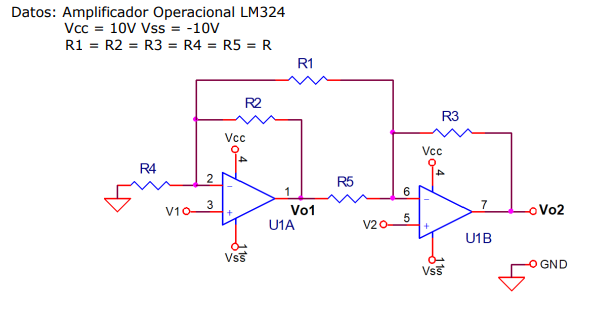
\includegraphics[width=1\textwidth]{figuras/circuito_consigna.png}
	\caption{Circuito propuesto}
\end{figure}
\subsection{Análisis teórico}
Se debe analizar la tensón de salida en función de la tensión de entrada en modo diferencial $ V_d=(V_2-V_1)$ y también en modo común $V_c=(V_1+V_2)/2$.\\
Para realizar el análisis en modo diferencial, se aplica el método de superposición, primero se calcula $V_{01}$ y luego $V_{02}$.

\subsubsection{Cálculo de $V_{01}$}
\onehalfspacing
\begin{flushleft}
\textbf{Pasivando $V_2$}\\
$V_{O1}|_{V_2=0}=(1+\frac{R}{R/2})V_1=3V_1$ \\
\textbf{Pasivando $V_1$} \\
$V_{O1}|_{V_1=0}=(-\frac{R}{R})V_2=-V_2$ 
\end{flushleft}\begin{center}
\boxed{V_{O1}=3V_1-V_2} 	
\end{center}

\subsubsection{Cálculo de $V_{02}$}
\begin{flushleft}
\textbf{Pasivando $V_1$ y $V_2$}\\
$V_{O2}|^{V_1=0}_{V_2=0}=(-\frac{R}{R})V_1=-V_{01}$ \\
\textbf{Pasivando $V_2$ y $V_{01}$} \\
$V_{O2}|^{V_2=0}_{V_{01}=0}=(-\frac{R}{R})V_1=-V_1$ \\
\textbf{Pasivando $V_1$ y $V_{01}$} \\
$V_{O2}|^{V_1=0}_{V_{01}=0}=(1+\frac{R}{R/2})V_2=3V_2$ 
\end{flushleft}
\begin{center}
	\boxed{V_{O2}=3V_2-V_1-3V_1+V_2=4V_2-4V_1=4(V_2-V_1)}\\
	reemplazando con $ V_d=(V_2-V_1)$ \\
	\boxed{V_{O2}=4V_d}
\end{center}
\begin{flushleft}
	Para el análisis en $V_c=(V_1+V_2)/2$ y haciendo $V_1=V_2$ tenemos que \begin{center}
		\boxed{V_{02}=0}
	\end{center}
\end{flushleft}
\subsubsection{Cálculo de RRMC}
\begin{center}
	$RRMC=(\frac{A_d}{A_c})=\frac{4}{0})$\\
	\boxed{RRMC=\infty}
\end{center}
\subsubsection{Respuesta en frecuencia}
En el Datasheet del LM324 se encuentra el dato de la $f_T=1[MHz]$ por lo tanto 
\begin{center}
	$\omega_T=2 \pi f_T$ \\
$\omega_H = \omega_T k = \omega_T \frac{1}{4} = \frac{\pi}{2} f_T $\\
$\omega_H = 1.57 [Mrps]$\\
$f_H = 250 [KHz]$
\end{center}
La ganancia del amplificador es 4 lo que se traduce en 12.04[dB]. A 250[KHz]  la ganancia disminuirá 3[dB], es decir que la amplitud quedará en 9.03[dB] ó 2.83 veces.
\begin{figure}[htb]
	\centering
			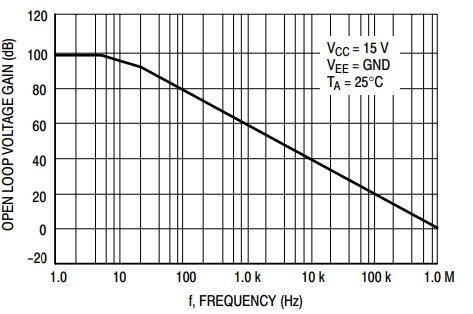
\includegraphics[width=0.6\textwidth]{figuras/graf_freq_lm324.png}
\end{figure}
\subsubsection{Impedancias}
Las impedancias vistas por las fuentes de señales $V_1$ y $V_2$ son las impedancias de entrada de ambos amplificadores. Definimos $Z_{i1}$ y $Z_{i2}$ a las impedancias vistas por $V_1$ y $V_2$ respectivamente.
\begin{center}
	$Z_{i1}= \frac{V_1}{I_{i1}}$ al ser $I_{i1}=0$ \\
	entonces queda $Z_{i1}= \infty$\\
	de manera análoga se determina\\
	 $Z_{i2}=\frac{V_2}{I_{i2}}=\infty$
\end{center}
\subsection{Simulaciones}
Se realizaron diferentes simulaciones con LTSpice para observar el comportamiento a la salida de cada amplificador. A continuación se listan las simulaciones realizadas:
\begin{itemize}
	\item $Vo_1$ y $Vo_2$ con $V_1=10[mV]$ y $V_2=0[mV]$.
	\item $Vo_1$ y $Vo_2$ con $V_1=0[mV]$ y $V_2=10[mV]$.
	\item $Vo_1$ y $Vo_2$ con $V_1 = V_2 = 10[mV]$ pero ambas entradas desfasadas 180° entre ellas.
	\item $Vo_1$ y $Vo_2$ con $V_1=V_2=10[mV]$ sin desfasar.
	\item Respuesta en frecuencia del circuito, graficando el Bode con Magnitud y Fase.
\end{itemize}
\begin{figure}[H]
	\centering
	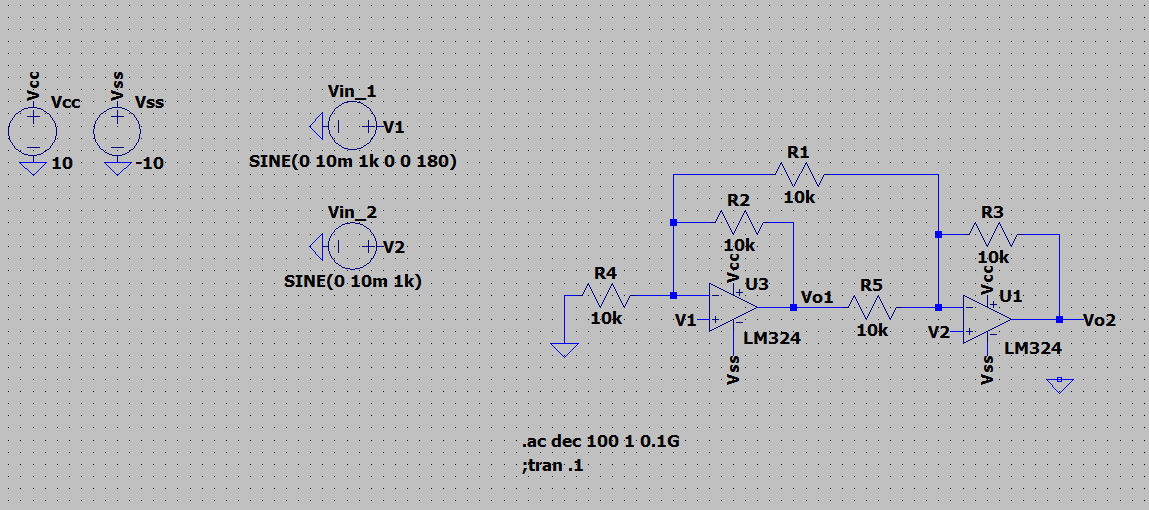
\includegraphics[width=1\textwidth]{figuras/circuito1.png}
	\caption{Circuito simulado}
\end{figure}
\begin{figure}[H]
	\centering
	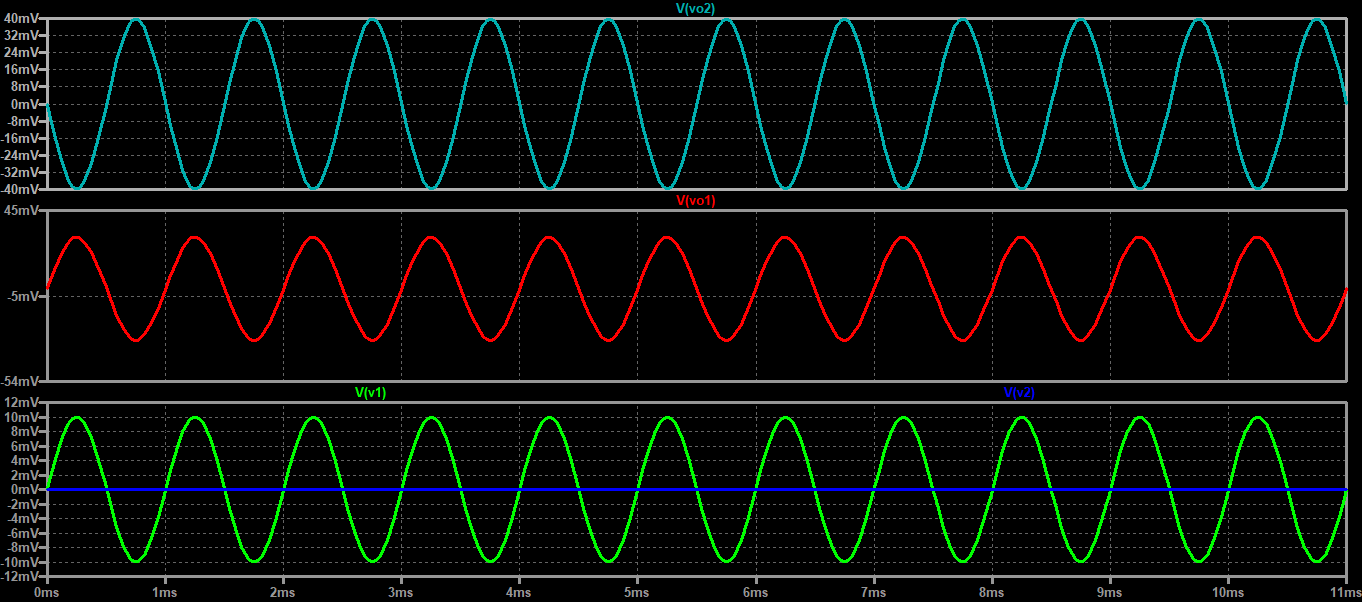
\includegraphics[width=1\textwidth]{figuras/Sim_V1=10mv_V2=0.png}
	\caption{$Vo_1$ (rojo) y $Vo_2$ (celeste) con $V_1=10[mV]$ y $V_2=0[mV]$.}
\end{figure}
\begin{center}
	\begin{tabular}{| c | c |}
	\hline
	   	& $V_1=10[mV]$ y $V_2=0[mV]$ \\ \hline
	$Vo_1$ 	&  	29.5 [mV]	 \\
	$Vo_2$ 	& 	39.73[mV]	 \\ \hline
\end{tabular}
	\end{center}

\begin{figure}[H]
	\centering
	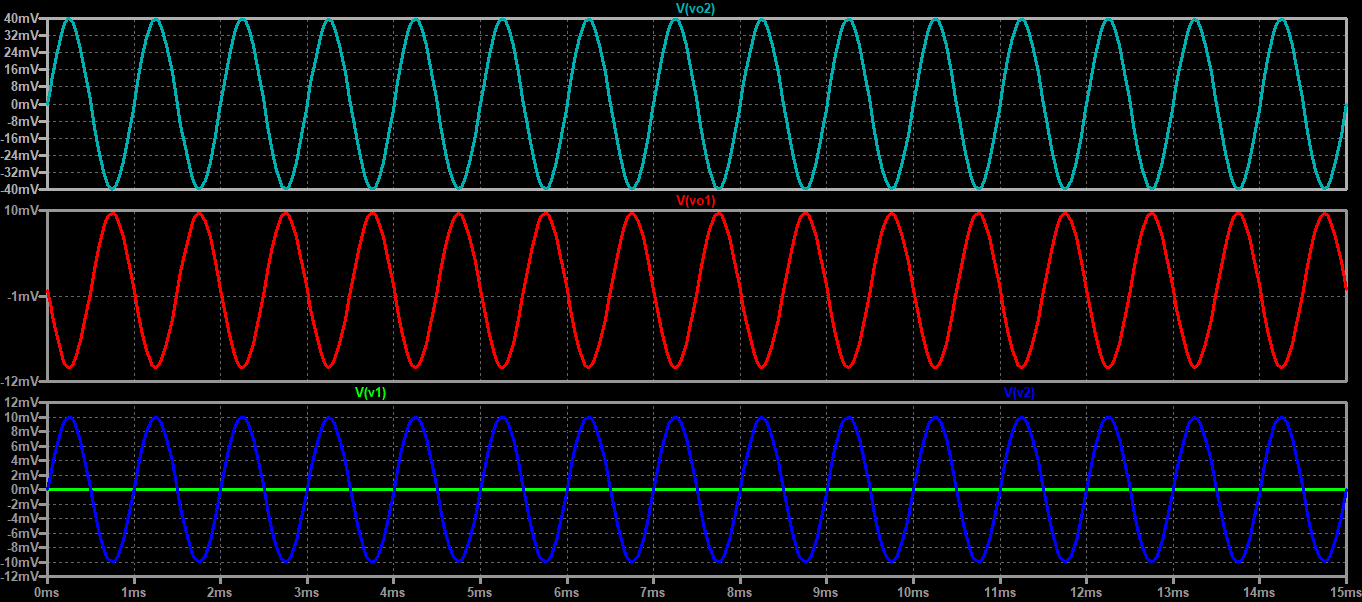
\includegraphics[width=1\textwidth]{figuras/Sim_V1=0_V2=10mv.png}
	\caption{$Vo_1$ (rojo) y $Vo_2$ (celeste) con $V_1=0[mV]$ y $V_2=10[mV]$.}
\end{figure}
\begin{center}
	\begin{tabular}{| c | c |}
		\hline
		& $V_1=0[mV]$ y $V_2=10[mV]$ \\ \hline
		$Vo_1$ 	&  	29.5 [mV]	 \\
		$Vo_2$ 	& 	39.73[mV]	 \\ \hline
	\end{tabular}
\end{center}

\begin{figure}[H]
	\centering
	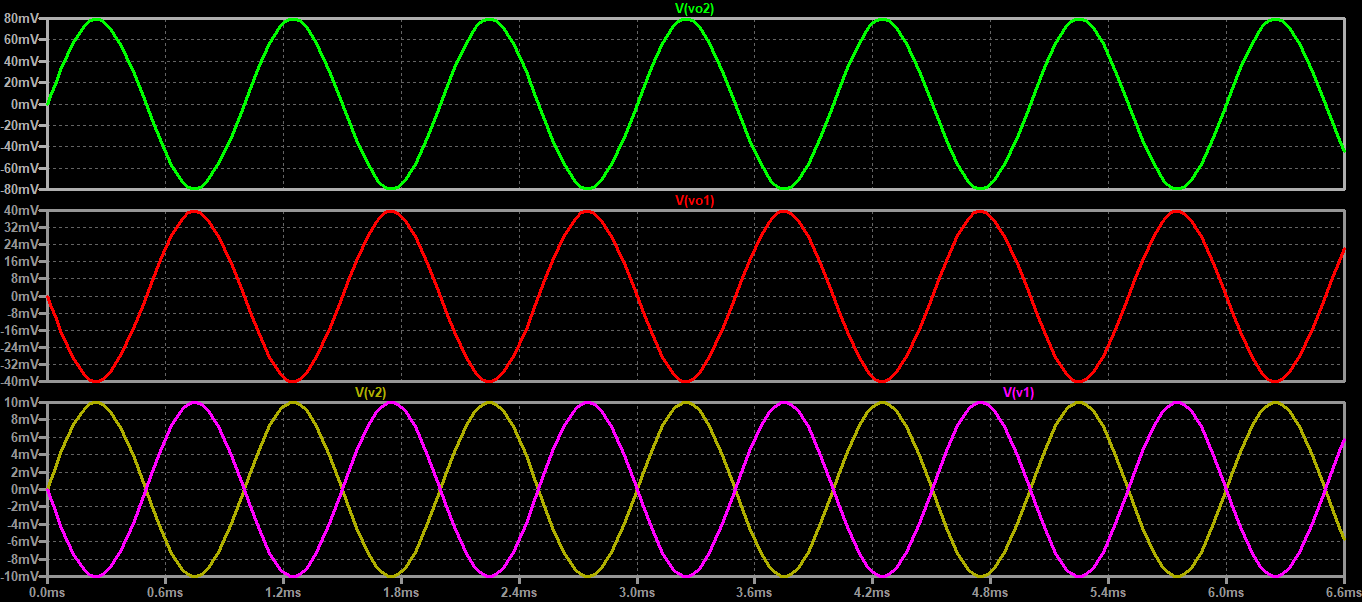
\includegraphics[width=1\textwidth]{figuras/Sim_Modo_Diferencial.png}
	\caption{$Vo_1$ (rojo) y $Vo_2$ (verde) con $V_1 = V_2 = 10[mV]$ pero ambas entradas desfasadas 180° entre ellas.}
\end{figure}
\begin{center}
	\begin{tabular}{| c | c |}
		\hline
		& $V_1=10[mV]$ y $V_2=10[mV]$ y $\Delta\varphi= 180$°\\ \hline
		$Vo_1$ 	&  	39.99 [mV]	 \\
		$Vo_2$ 	& 	79.46[mV]	 \\ \hline
	\end{tabular}
\end{center}
\begin{figure}[H]
	\centering
	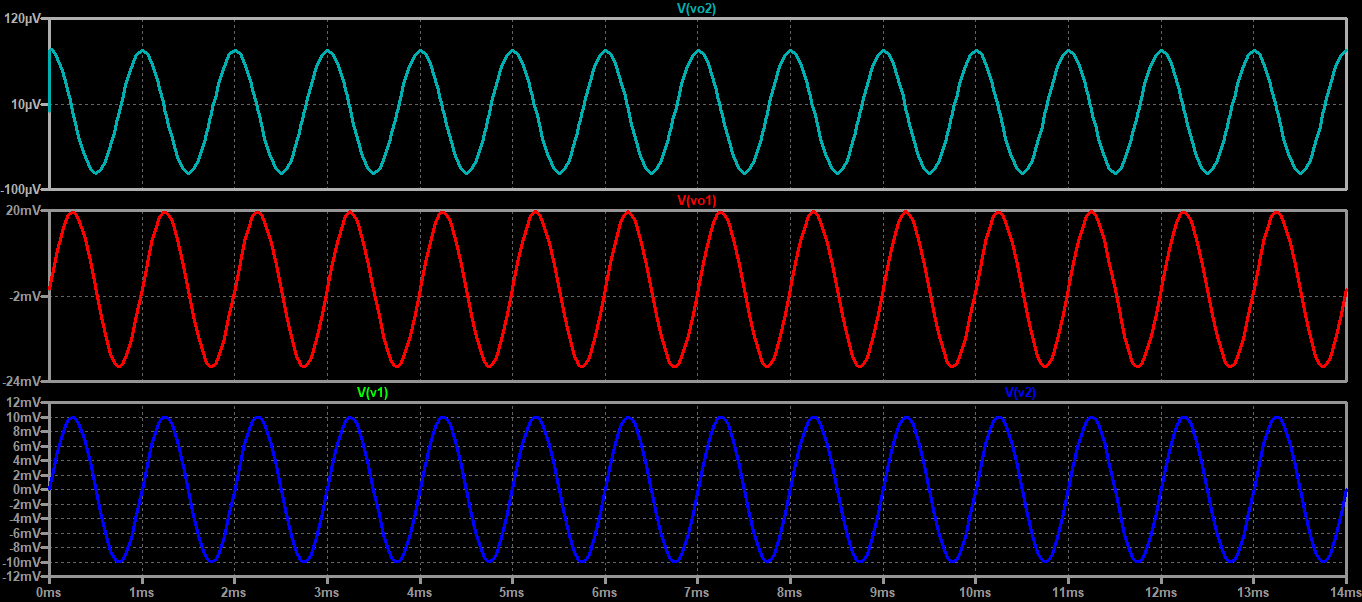
\includegraphics[width=1\textwidth]{figuras/Sim_Modo_Comun.png}
	\caption{$Vo_1$ (rojo) y $Vo_2$ (celeste) con $V_1=V_2=10[mV]$ sin desfasar.}
\end{figure}
\begin{center}
	\begin{tabular}{| c | c |}
		\hline
		& $V_1=10[mV]$ y $V_2=10[mV]$ y $\Delta\varphi= 0$\\ \hline
		$Vo_1$ 	&  	19.60 [mV]	 \\
		$Vo_2$ 	& 	79.14[\textmu V]	 \\ \hline
	\end{tabular}
\end{center}
\begin{figure}[H]
	\centering
	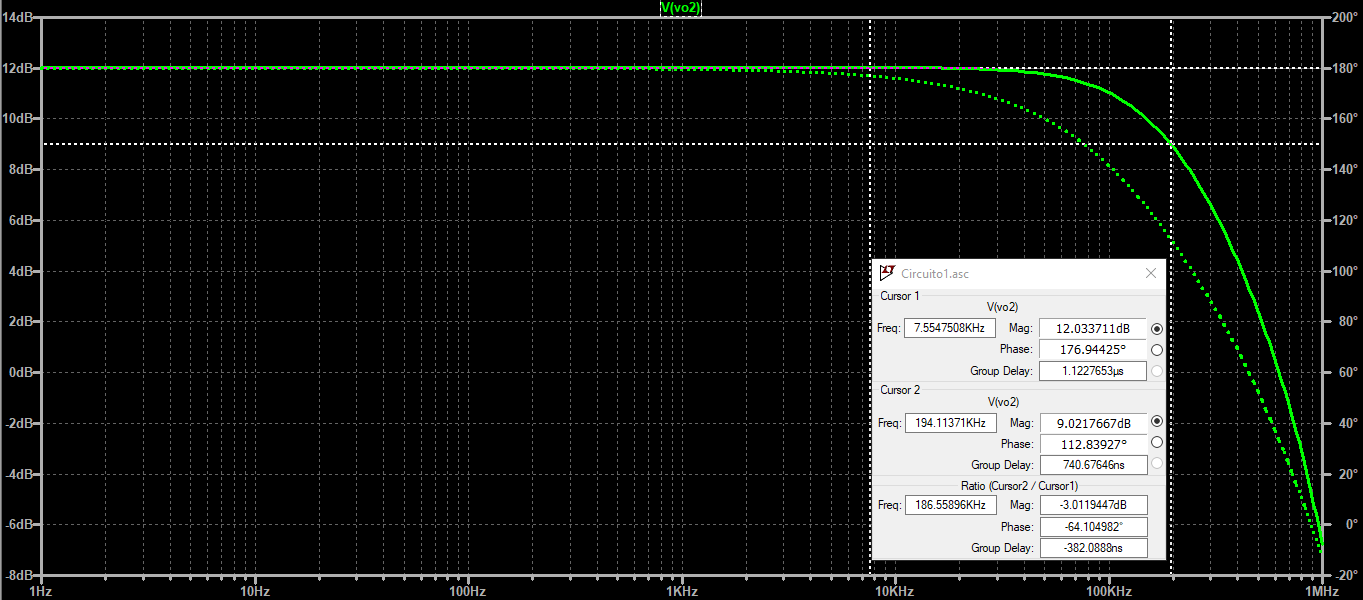
\includegraphics[width=1\textwidth]{figuras/lab1_freq.png}
	\caption{Bode con Magnitud y Fase -$Vo_2$ con $V_1=1[V]$ y $V_2=0[V]$.}
\end{figure}
\begin{center}
	\begin{tabular}{| c | c |}
		\hline
		& $V_1=1[V]$ y $V_2=0[V]$ \\ \hline
		Frecuencia para -3[dB] 	&  	186.55 [KHz]	 \\
		$\Delta\varphi$ 	& 	64.10°	 \\ \hline
	\end{tabular}
\end{center}
\subsection{Implementación}


\subsection{Comparación entre resultados}
En la siguiente tabla comparativa se reflejan los resultados obtenidos en cada una de las etapas previas y se calcula el error relativo que existe entre los resultados.\\
Tanto para la simulación como para la parte experimental, se ingresó señal por $V_1$
\begin{table}[H]
	\begin{center}
		\begin{tabular}{| c | c | c | c | c |c |c |}
			\hline
			& \multicolumn{3}{ |c| }{Salida $Vo_2$[V]} &
			\multicolumn{3}{ |c| }{Errores relativos (\%)} \\ \hline
			Entrada $V_1$[V] & Teoría & Simulación & Experimental & Exp/Teo & Exp/Sim & Sim/Teo \\ \hline
			0.2 & 0.8 & 0.7989	& - & - & - & 0.14 \\
			0.4 & 1.6 & 1.5973	& - & - & - & 0.17 \\
			1   &  4  & 3.9974	& - & - & - & 0.06 \\ \hline
		\end{tabular}
	\end{center}
\end{table} 

\subsection{Conclusión}
Se puede concluir que la herramienta de simulación es bastante precisa, pues el error relativo respecto al valor teórico siempre se mantuvo menor al 1\%.\\
Ahora bien, el error relativo entre el valor teórico y el experimental es mas grande, aproximadamente (...\%), esto se debe a que los componentes no son ideales y el comportamiento puede variar en un rango acotado indicado por el fabricante.  

	\newpage
\section{Fuente de corriente controlada por tensión}
\onehalfspacing
\begin{figure}[htb]
	\centering
	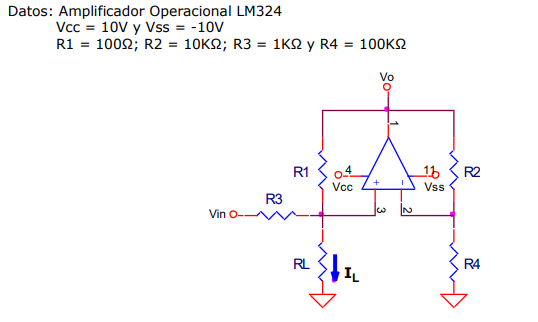
\includegraphics[width=1\textwidth]{figuras/circuito2_consigna.png}
	\caption{Circuito propuesto}
\end{figure}
\subsection{Análisis teórico}



\subsection{Simulaciones}
Se realizaron diferentes simulaciones con LTSpice para observar el comportamiento a la salida de cada amplificador. A continuación se listan las simulaciones realizadas:
\begin{itemize}
	\item ...
	\item ...
	\item ...
\end{itemize}
\begin{figure}[H]
	\centering
	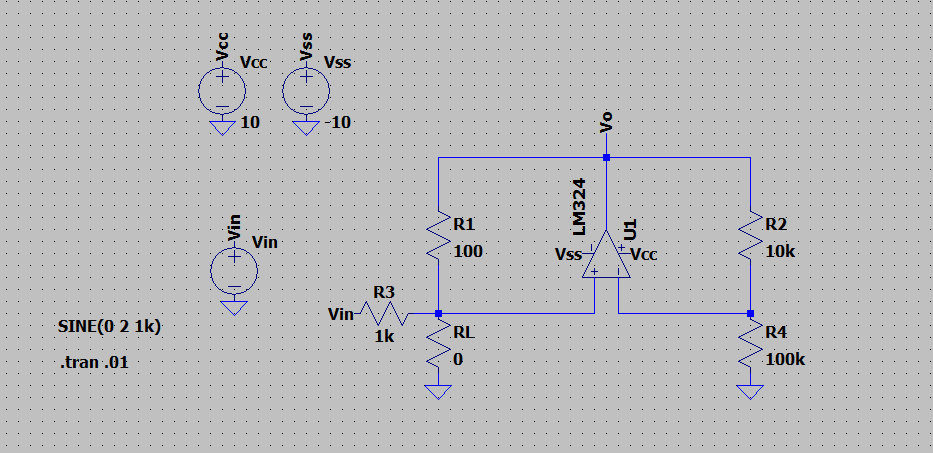
\includegraphics[width=1\textwidth]{figuras/circuito2.png}
	\caption{Circuito simulado}
\end{figure}

\subsection{Implementación}


\subsection{Comparación entre resultados}

\subsection{Conclusión}
 
\end{document}
